\documentclass[12pt,a4paper]{report} 
\usepackage[utf8]{inputenc}
\usepackage{background}
\usepackage{style/XThesis2} 
\usepackage{xcolor}
\usepackage{natbib}
\usepackage{url}
\usepackage{enumerate}
\usepackage{caption}
\usepackage{float}
\usepackage[section]{placeins}
\usepackage{times}
\usepackage{graphicx}
\usepackage{algorithmic}
\usepackage{amsmath, amsthm, amssymb}
\usepackage{subfigure}
\usepackage{url}
\usepackage[encapsulated]{CJK} 
\usepackage[nottoc,notlot,notlof]{tocbibind}


\backgroundsetup{
scale=1.5
,
contents= {
\includegraphics{images/nthu_logo}}
}
%-------------------------------------------------------------------------
% take the % away on next line to produce the final camera-ready version
\pagestyle{empty}

%-------------------------------------------------------------------------
\begin{document}
\begin{CJK}{UTF8}{bsmi}



\beforepreface 

%-------------------------------------------------------------------------
\clearpage\maketitle
\thispagestyle{empty}
%-------------------------------------------------------------------------

\afterpreface 




\chapter{Introduction}
    Firstly we introduce the situation that graduate students are struggling with their research.
    
    \begin{figure}[H]
    
        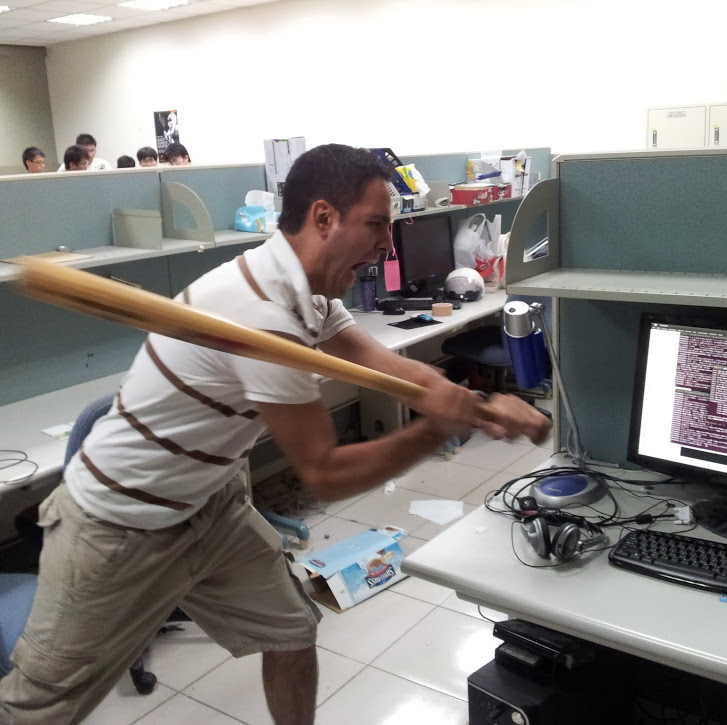
\includegraphics[scale=0.35]{images/frustrated_student.jpg}
        \caption{A student is resolving his graduation anxiety to violence.}
        \label{fig:student}
    \end{figure}
    



\chapter{Related Work}
    Many researchers have been studying graduate students, one of them are Madsen et al\citep{madsen1992successful}
 
\chapter{Method}
    We use a simple regression model approach to predict the graduation time of a student.
    \begin{figure}[H]
    
        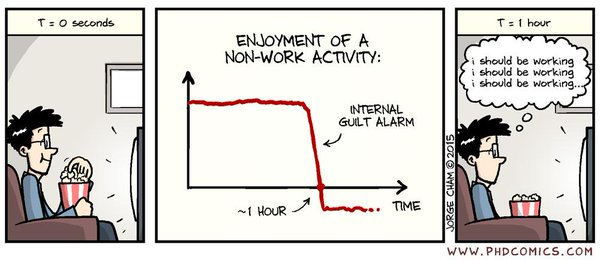
\includegraphics[scale=0.65]{images/phd_comic.jpg}
        \caption{A typical syndrome most of the graduate students have.}
        \label{fig:phd_comic}
    \end{figure}
    


\chapter{Experiment}
The "X" has won!
    \begin{center}
        \begin{tabular}{ |c|c|c| } 
             \hline
             X & O & O \\ 
              \hline
             O & X & O \\ 
              \hline
             X & O & X \\ 
             \hline
        \end{tabular}
        \captionof{table}{A Tic Tac Toe game.}\label{table:tic_tac_toe}
    \end{center}
 





\chapter{Conclusion}
    We conclude that the time of graduation is totally depends on the student him/her self. 

\end{CJK}

\bibliographystyle{plain}
\bibliography{rreferences}
\end{document}
